\documentclass[10pt]{beamer}
\usetheme{Malmoe}
\colorlet{beamer@blendedblue}{green!40!black}
\setbeamertemplate{navigation symbols}{}
\newcommand*\oldmacro{}%
\let\oldmacro\insertshorttitle%
\renewcommand*\insertshorttitle{%
\oldmacro\hfill%
\insertframenumber\,/\,\inserttotalframenumber}

\usepackage{caption}
\usepackage{hyperref}
\usepackage[makeroom]{cancel}
\usepackage{ amssymb }
\usepackage{appendixnumberbeamer}
%\usepackage{tikz-feynman}
\usepackage{graphicx}
\begin{document}
\title{Search for Flavor Changing Neutral Currents in Top Quark Decays}
\subtitle{$t \rightarrow q \gamma$}
\author[Barkeloo]{Jason Barkeloo}

\titlegraphic{
\includegraphics[width=4cm]{../ATLAS-Logo-Ref-RGB.png}\hspace*{2.75cm}~%
   
\includegraphics[width=4cm]{../uo_logo_green_on_white_2.jpg}
}

%\frame{\frametitle{}
%\begin{itemize}
%\item
%\end{itemize}
%}


\date{July 11, 2019}
\frame{\titlepage}
\frame{\frametitle{Overview}\tableofcontents[]}%hidesubsections]}
\section{Brief Background}
%\frame{\frametitle{Table of Contents}\tableofcontents[currentsection,hideothersubsections]}
%%%%%%%%%%%%%%%%%%%%%%%%%%%%%%%%%%%%%%%%%%%%%%%%%%%%%%%%%

\subsection{The Top Quark}

\frame{\frametitle{Top Quark Decays in the SM}
\centering
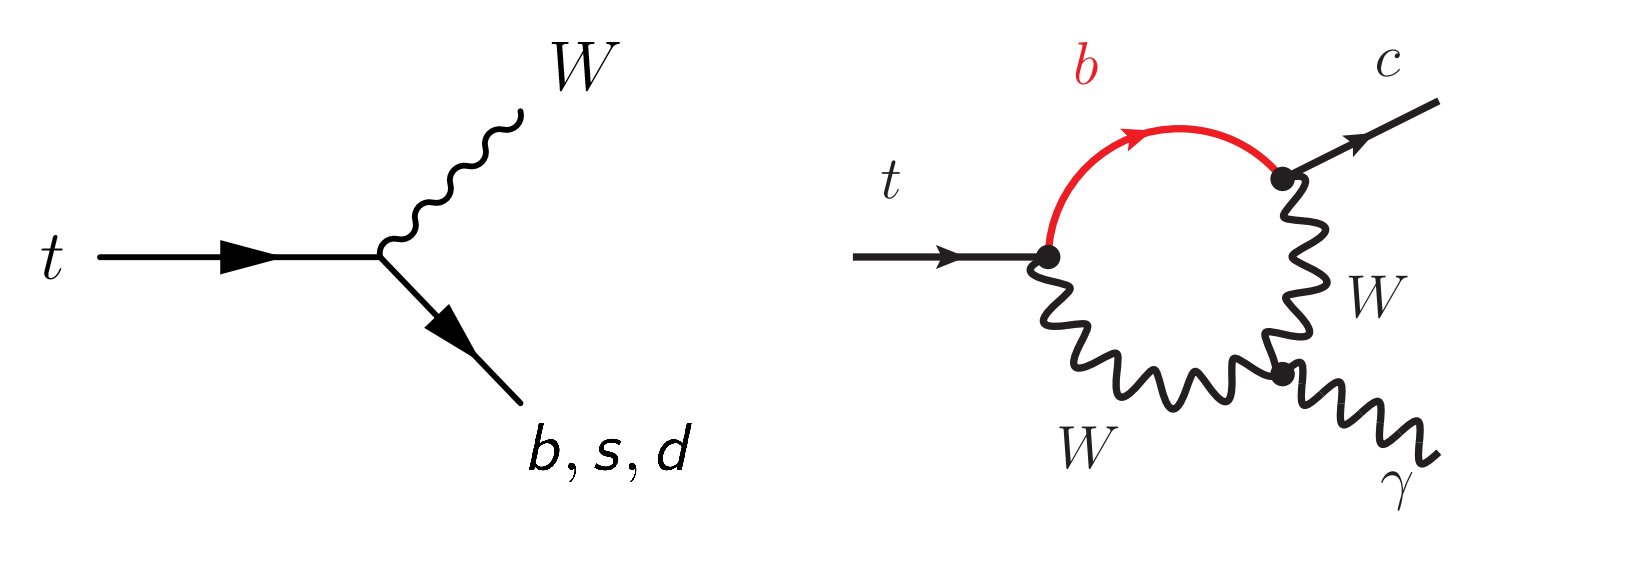
\includegraphics[width=1.\textwidth]{../../Thesis/ThesisImages/SMTopDecays2.png}

\begin{columns}
\begin{column}{0.5\textwidth}
\begin{itemize}
\item $t\rightarrow b W \approx 99.83\%$
\item $t\rightarrow s W \approx 0.16\%$
\item $t\rightarrow d W \approx 0.01\%$
\end{itemize}
\end{column}
\begin{column}{0.5\textwidth}
\begin{itemize}
\item $t\rightarrow q_{u,c} X\approx 10^{-17} - 10^{-12}$
\item Limits on $t\rightarrow \gamma q$ processes: \href{https://arxiv.org/abs/1511.03951}{[JHEP 04 (2016) 035]}
	\begin{itemize}
	\item $t\rightarrow \gamma u < 1.3 x10^{-4}$
	\item $t\rightarrow \gamma c < 1.7 x 10^{-3}$
	\end{itemize}
\end{itemize}
\end{column}
\end{columns}
}



\subsection{FCNC at the LHC} 

\frame{\frametitle{FCNC: What are we looking for? $t\bar{t}\rightarrow W (\rightarrow l \nu) b+ q\gamma$}
\begin{itemize}
\item Final state topology
	\begin{itemize}
	\item One Neutrino, from W
	\item One Lepton, from W
	\item One B-jet, SM Top
	\item One Photon, FCNC Top
	\item One Jet, FCNC Top
	\end{itemize}
\end{itemize}
\centering
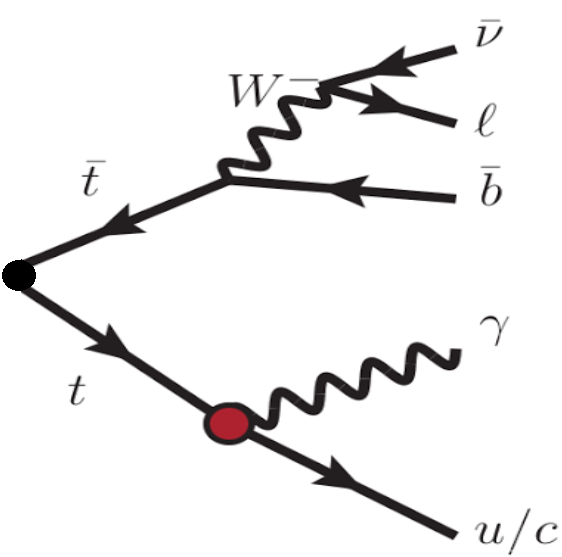
\includegraphics[width=0.4\textwidth]{../../Thesis/ThesisImages/fcncttbar.png}
}

%%%%%%%%%%%%%%%%%%%%%%%%%%%%%%%%%%%%%%%%%%%%%%%%%%%%%%%%%%%%%%%%%

\subsection{Object Preselection Cuts}


\frame{\frametitle{Object Preselection}
\begin{itemize}
\item We preselect events with objects that look like similar to our expected topology
\item Require:
	\begin{itemize}
	\item Exactly one lepton (e or $\mu$) $\geq$ 25 GeV
	\item Exactly one good photon $\geq$ 15GeV
	\item Missing Transverse Energy $\geq$ 30GeV
	\item $\geq 2$ Jets (at least 1 b-tag)
	\end{itemize}
\item Plots shown will be with MC16a and Data15/16 (36.2 $\text{fb}^{-1}$)

\end{itemize}
}



\frame{\frametitle{Preselection Objects with $N_{BJet}= 1$ }
\begin{columns}
\begin{column}{0.02\textwidth}
\rotatebox{90}{Muon Channel \qquad  Electron Channel} 
%\rotatebox{90}{Muon Channel        } 
\end{column}
\begin{column}{0.33\textwidth}
\begin{itemize}
\item  Leading Jet $p_T$
\end{itemize}
%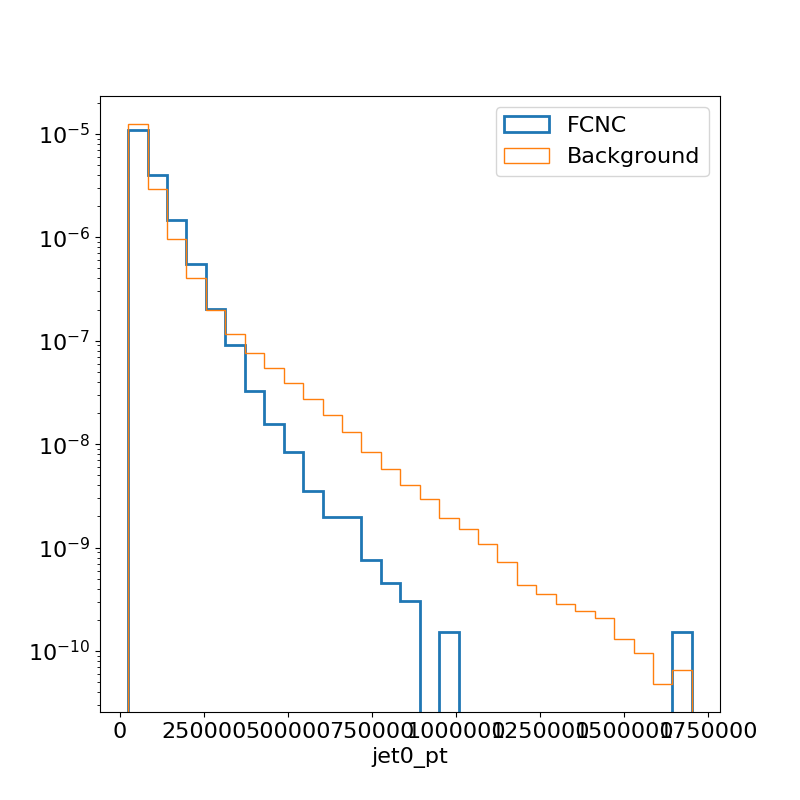
\includegraphics[width=.85\textwidth]{Images/ejetsvarplots/jet0_pt.png} \\
%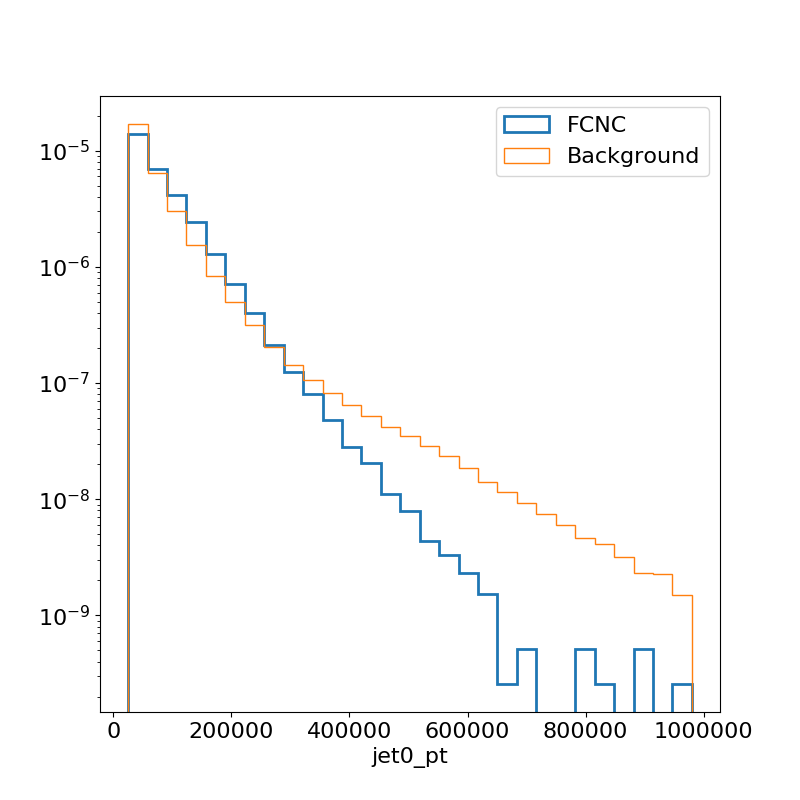
\includegraphics[width=.85\textwidth]{Images/mujetsvarplots/jet0_pt.png}
\end{column}
\begin{column}{0.33\textwidth}
\begin{itemize}
\item Lead Photon
\end{itemize}
%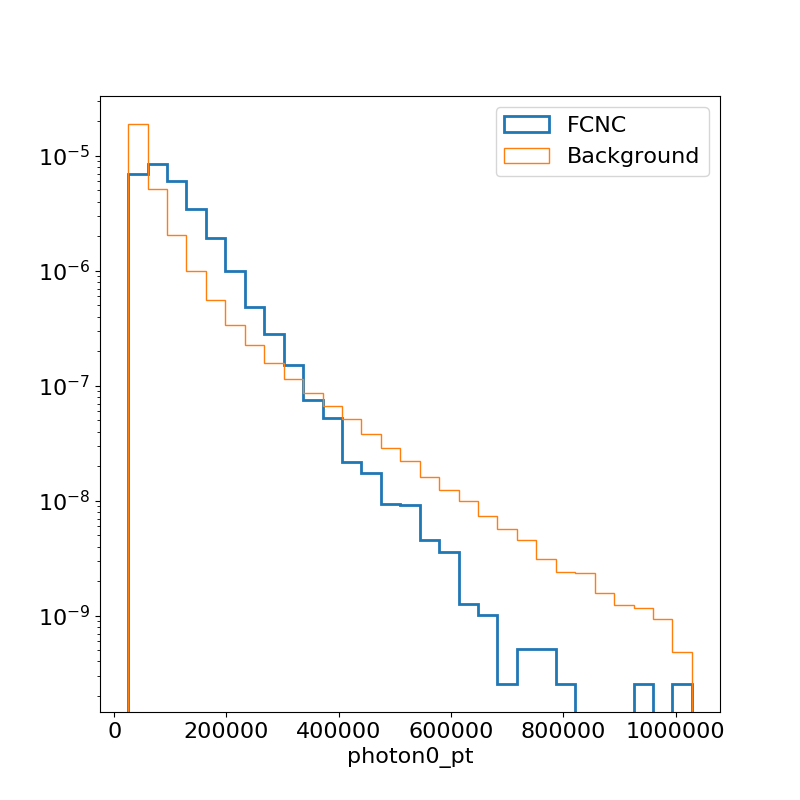
\includegraphics[width=.85\textwidth]{Images/ejetsvarplots/photon0_pt.png} \\
%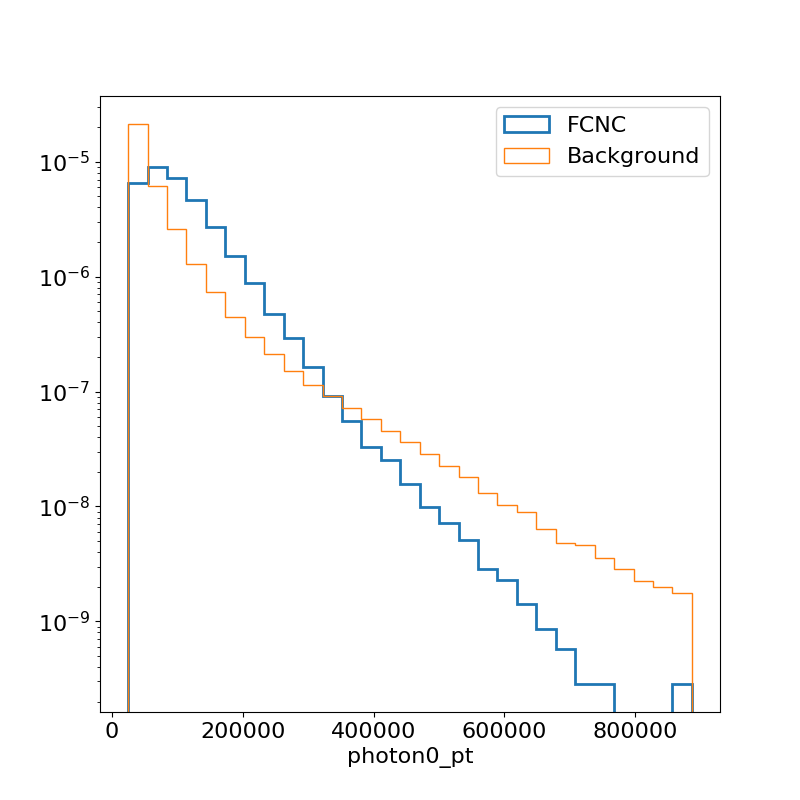
\includegraphics[width=.85\textwidth]{Images/mujetsvarplots/photon0_pt.png}
\end{column}
\begin{column}{0.33\textwidth}
\begin{itemize}
\item Lepton E
\end{itemize}
%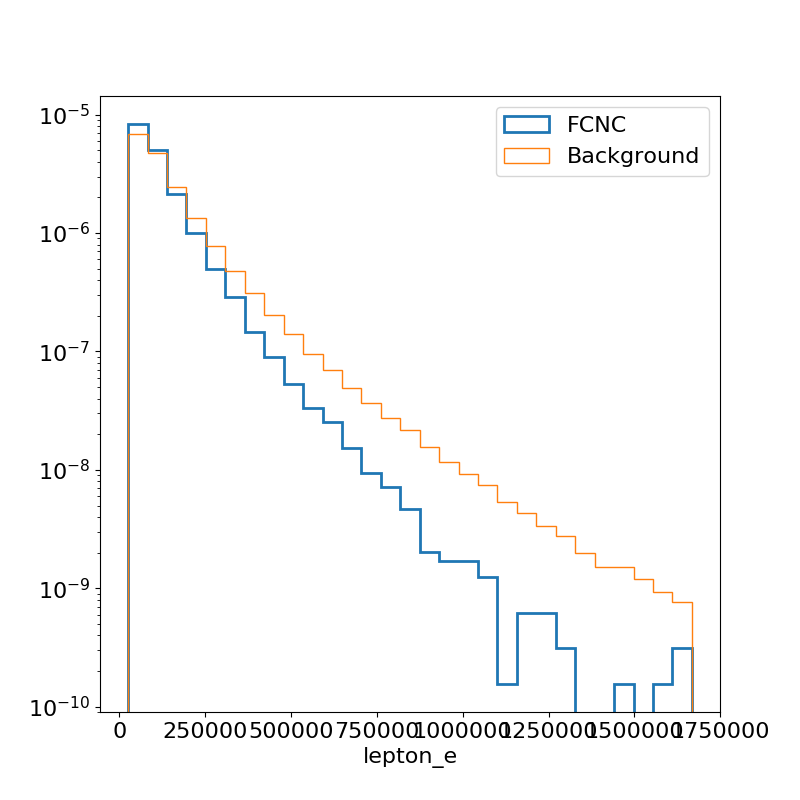
\includegraphics[width=.85\textwidth]{Images/ejetsvarplots/lepton_e.png} \\
%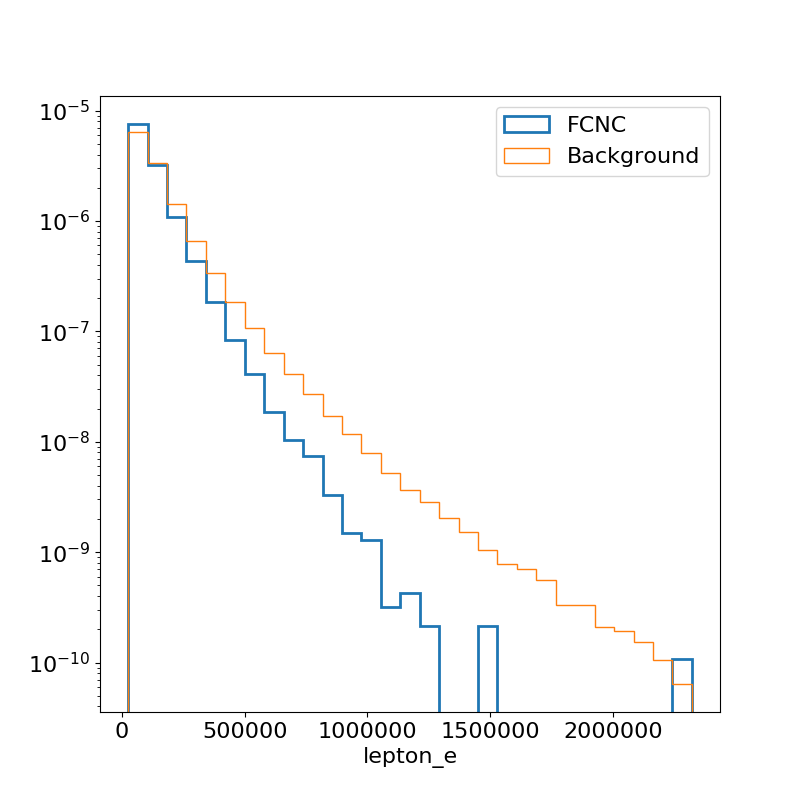
\includegraphics[width=.85\textwidth]{Images/mujetsvarplots/lepton_e.png}
\end{column}
\end{columns}
}

%\frame{\frametitle{Preselection Objects with $N_{BJet}= 1$ }
%\begin{columns}
%\begin{column}{0.02\textwidth}
%\rotatebox{90}{Muon Channel \qquad  Electron Channel} 
%%\rotatebox{90}{Muon Channel        } 
%\end{column}
%\begin{column}{0.33\textwidth}
%\begin{itemize}
%\item $\gamma_{iso}$
%\end{itemize}
%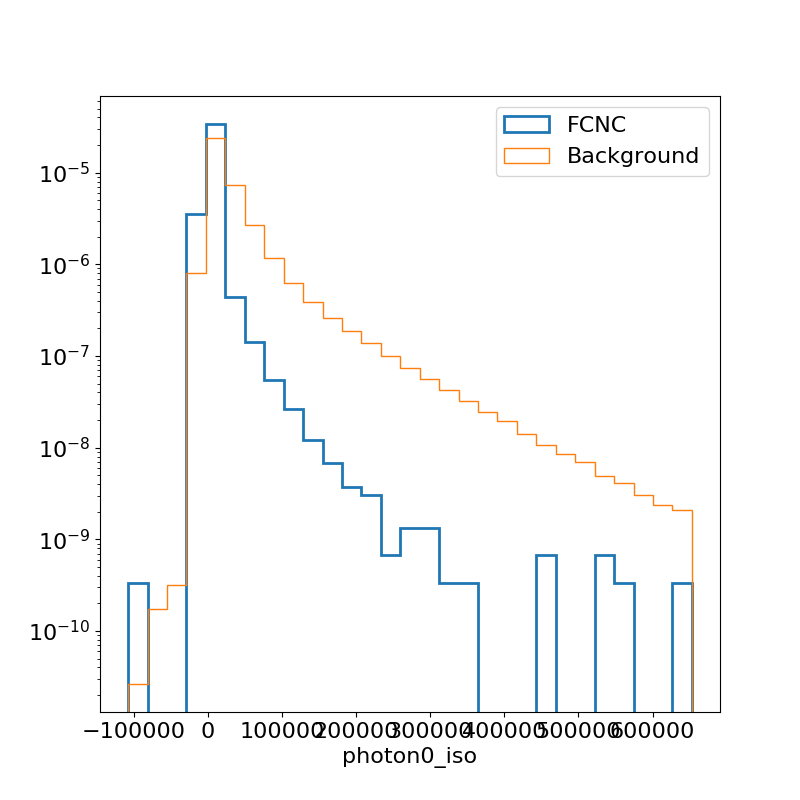
\includegraphics[width=.85\textwidth]{Images/ejetsvarplots/photon0_iso.png} \\
%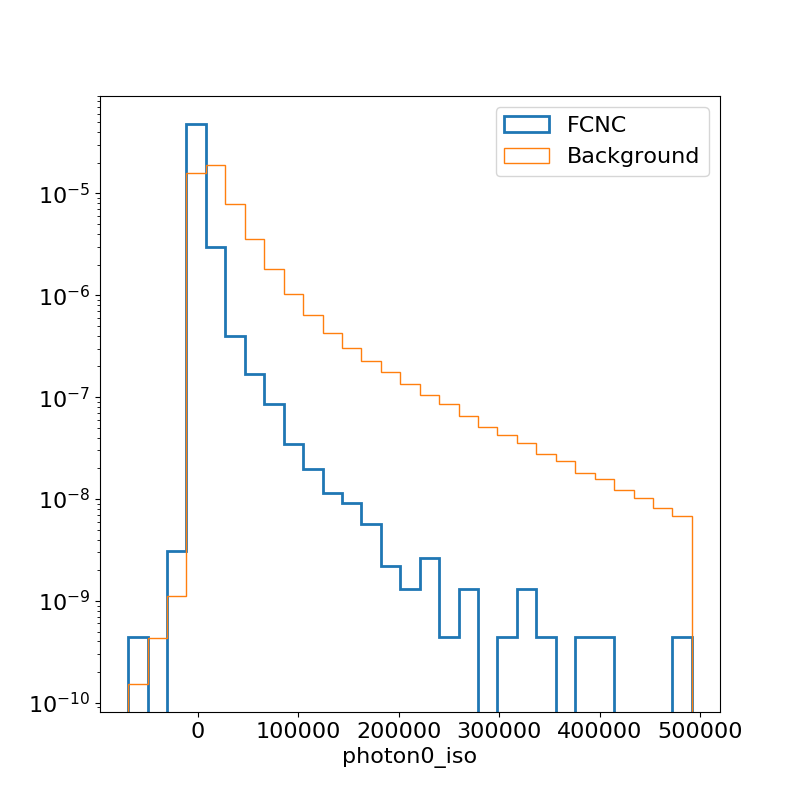
\includegraphics[width=.85\textwidth]{Images/mujetsvarplots/photon0_iso.png}
%\end{column}
%\begin{column}{0.33\textwidth}
%\begin{itemize}
%\item $\Delta R_{j\gamma}$
%\end{itemize}
%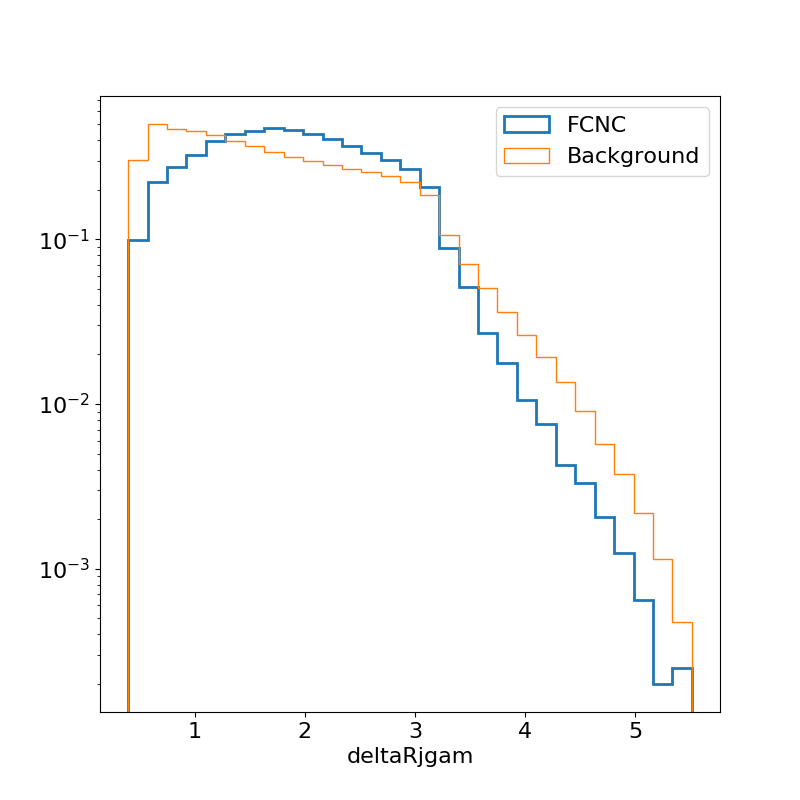
\includegraphics[width=.85\textwidth]{Images/ejetsvarplots/deltaRjgam.png} \\
%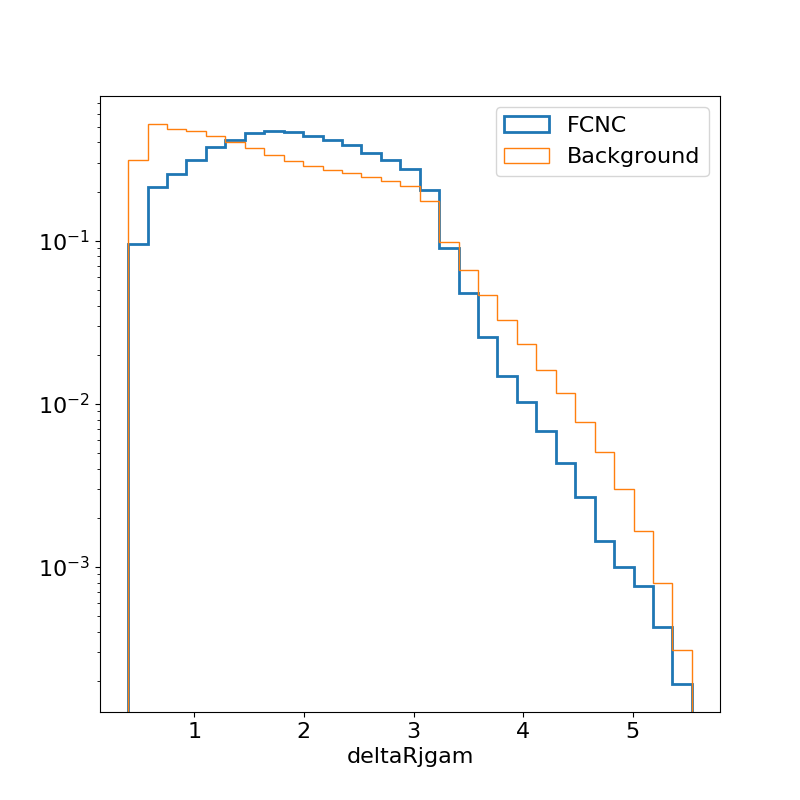
\includegraphics[width=.85\textwidth]{Images/mujetsvarplots/deltaRjgam.png}
%\end{column}
%\begin{column}{0.33\textwidth}
%\begin{itemize}
%\item $\Delta R_{l\gamma}$
%\end{itemize}
%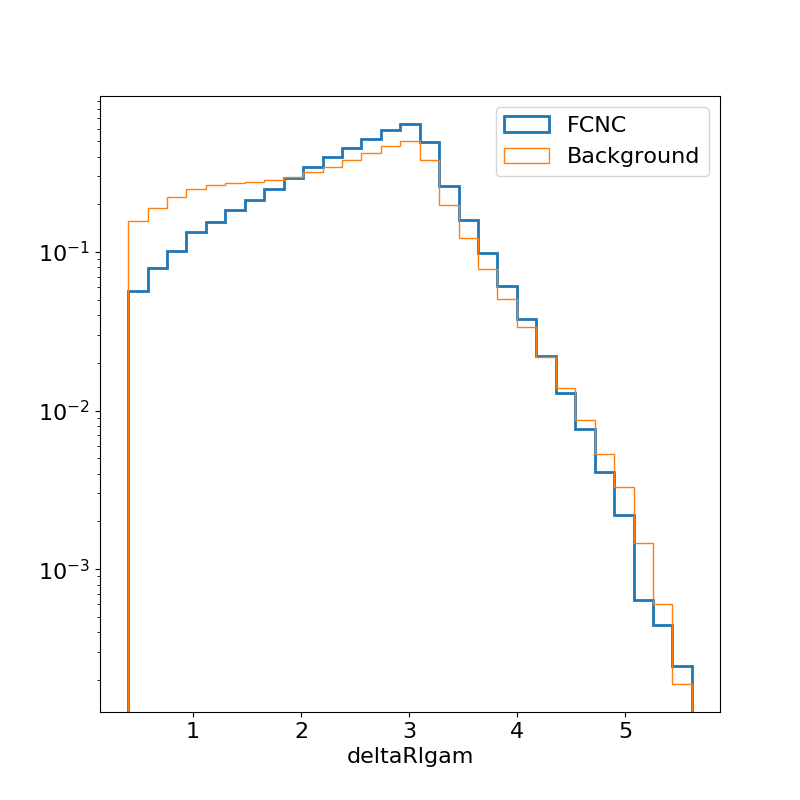
\includegraphics[width=.85\textwidth]{Images/ejetsvarplots/deltaRlgam.png} \\
%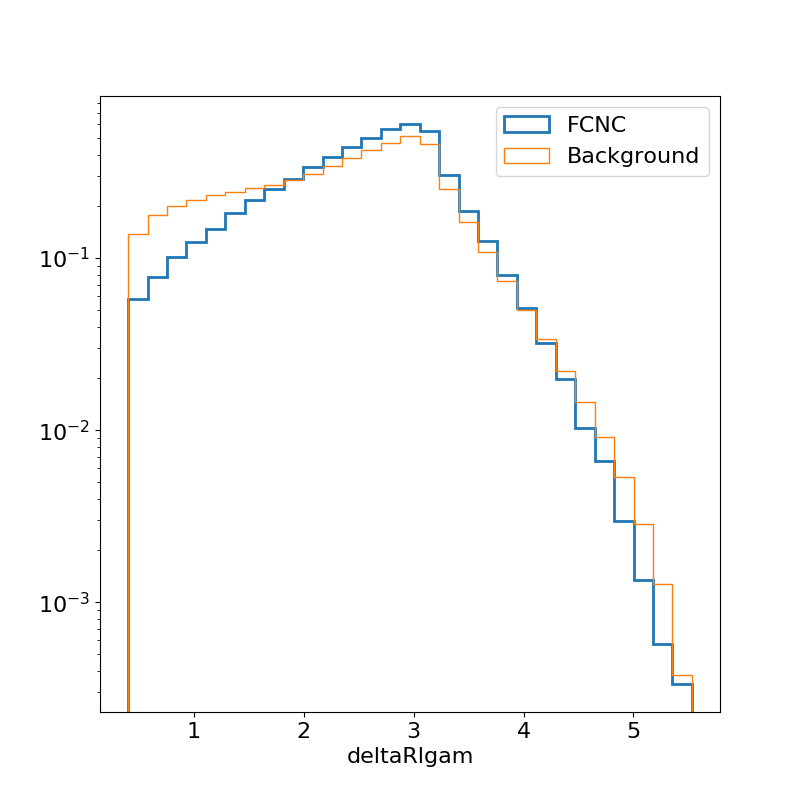
\includegraphics[width=.85\textwidth]{Images/mujetsvarplots/deltaRlgam.png}
%\end{column}
%\end{columns}
%}


%%%%%%%%%%%%%%%%


\section{Neural Network}
\subsection{Neural Network Studies}

\frame{\frametitle{Neural Network Architecture}
\begin{itemize}
\item Using Keras on top of Tensorflow various input parameters are tested for model behavior
\item A Dense Neural Network with variable number of input variables and hidden layers are explored
\item Cut optimization has been performed with full Run 2 luminosity for potential reach of the search
\end{itemize}
\centering
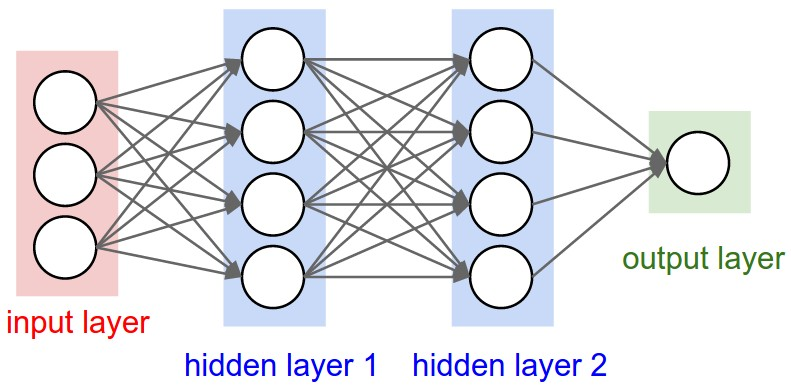
\includegraphics[width=0.7\textwidth]{Images/neural_net2.jpeg}
\captionof{figure}{\href{http://cs231n.github.io/neural-networks-1/}{[Ref: Neural Network]}}
}

\frame{\frametitle{Neural Network Model Inputs}
\begin{itemize}
\item Using keras on top of tensorflow various input parameters are tested for model behavior
\item Networks are set up with 1 input layer, 2 hidden layers with 10 nodes (+1 bias node) \href{https://www.quora.com/What-is-bias-in-artificial-neural-network}{[Ref: Bias]}, and 1 output node
\item Each hidden layer has 20\% dropout to prevent overtraining by removing codependency between nodes
\item Batch size of 100 used and each network is allowed 200 epochs (with patience=50), all models converge and end early with reasonable batch sizes
\item Optimizer: Adam
\item Loss Function: Binary Cross Entropy
\item Many sets of input variables tested, best results from follow-up studies shown
\end{itemize}
}

\frame{\frametitle{Cut Optimization}
\begin{itemize}
\item Follow up changes allow a better limit with a cut that is slightly less harsh (0.96/0.95 instead of 0.98)
\item Estimated limit reduced by a factor of 2 by reweighting the number of events the model saw by taking advantage of the loss function
\[\text{Loss} = -\frac{1}{N}\sum_{i=1}^{N}y_{i} \text{log}(p(y_{i}))+(1-y_{i})\text{log}(1-p(y_{i}))\]
\item y - binary indicator (0 or 1) if class label is the correct classification for observation 
\item p - predicted probability observation is the class label (0 or 1)
\end{itemize}
} 

\frame{\frametitle{Neural Network Separation}
\begin{columns}
\begin{column}{0.02\textwidth}
\rotatebox{90}{Muon Channel \qquad Electron Channel \qquad} 
%\rotatebox{90}{Muon Channel        } 
\end{column}
\begin{column}{0.48\textwidth}
\begin{itemize}
\item  Previous
\end{itemize}
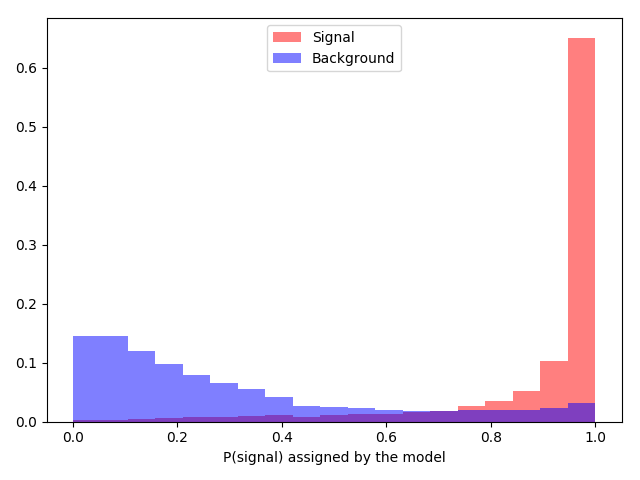
\includegraphics[width=.85\textwidth]{Images/previousEJetOuts/sigbkg.png} \\
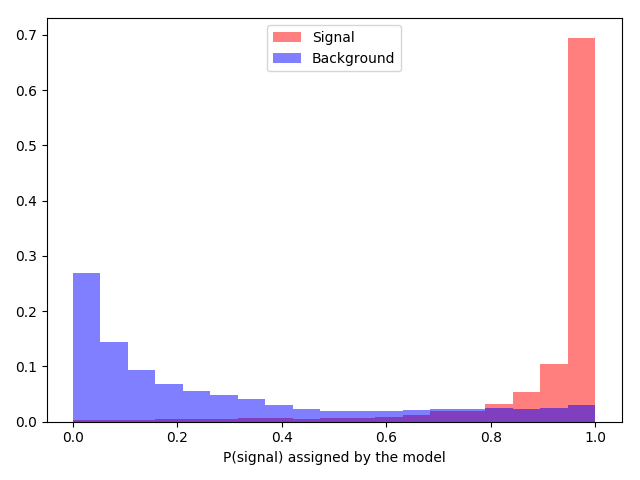
\includegraphics[width=.85\textwidth]{Images/previousMuJetOuts/sigbkg.png}
\end{column}
\begin{column}{0.48\textwidth}
\begin{itemize}
\item Current
\end{itemize}
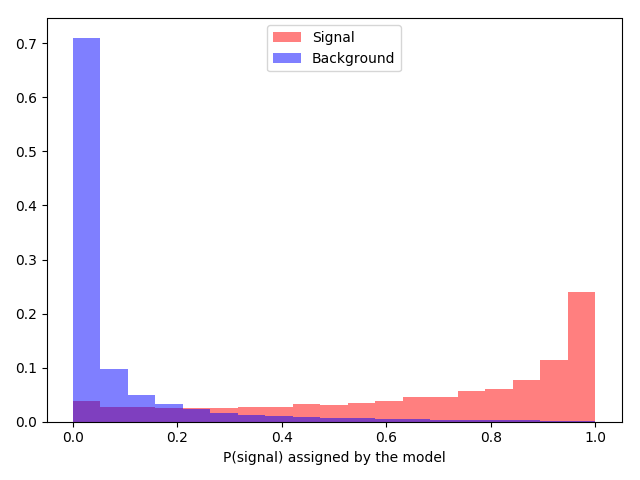
\includegraphics[width=.85\textwidth]{Images/ejetsOuts/sigbkg.png} \\
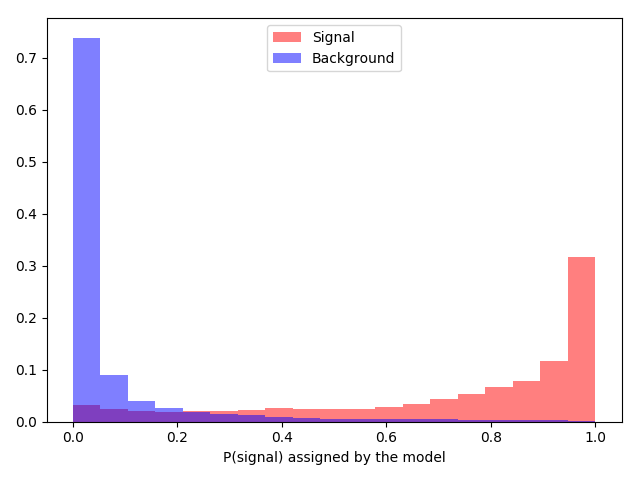
\includegraphics[width=.85\textwidth]{Images/mujetsOuts/sigbkg.png}
\end{column}
\end{columns}
}



\frame{\frametitle{Significance Plots, Electron Channel}
\begin{columns}
\begin{column}{0.48\textwidth}
\centering
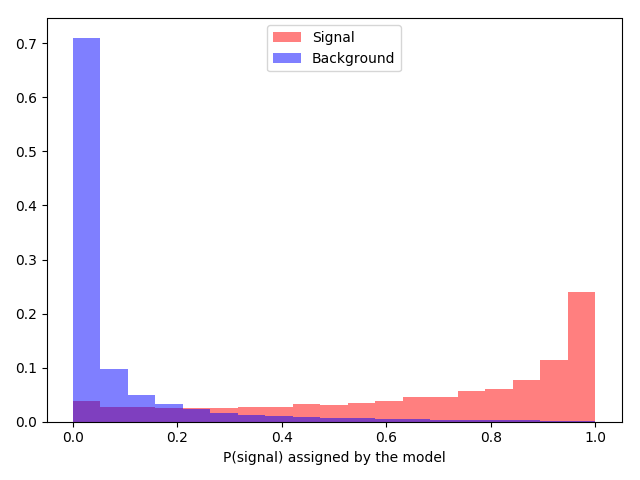
\includegraphics[width=0.85\textwidth]{Images/ejetsOuts/sigbkg.png} 
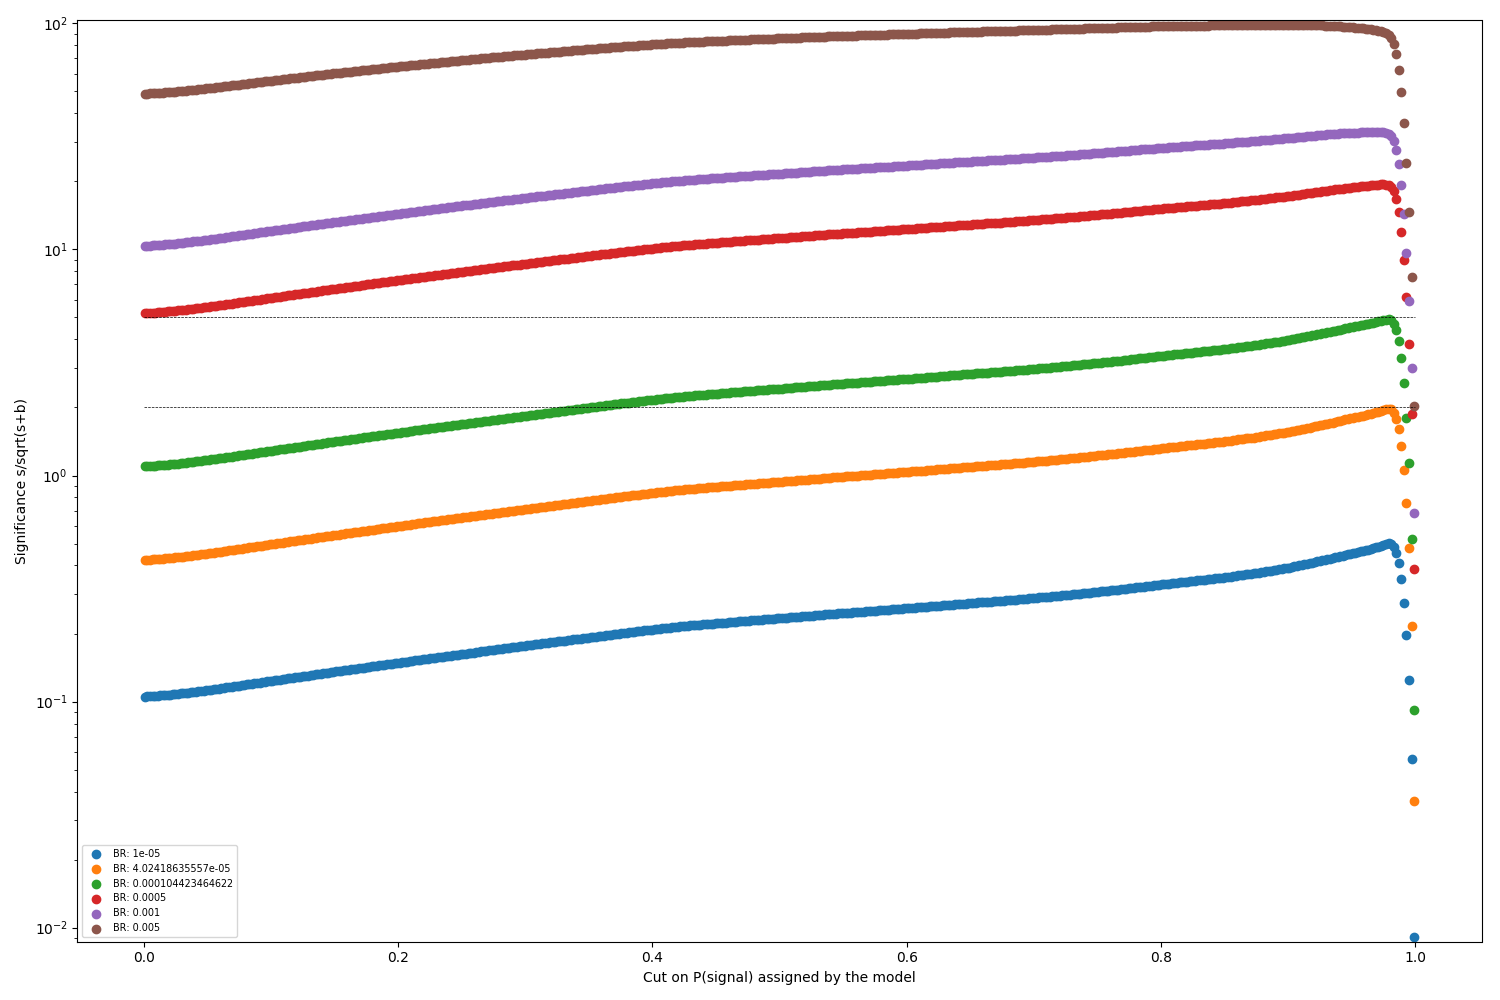
\includegraphics[width=0.85\textwidth]{Images/ejetsOuts/significance2.png} 
\end{column}
\begin{column}{0.48\textwidth}
\centering
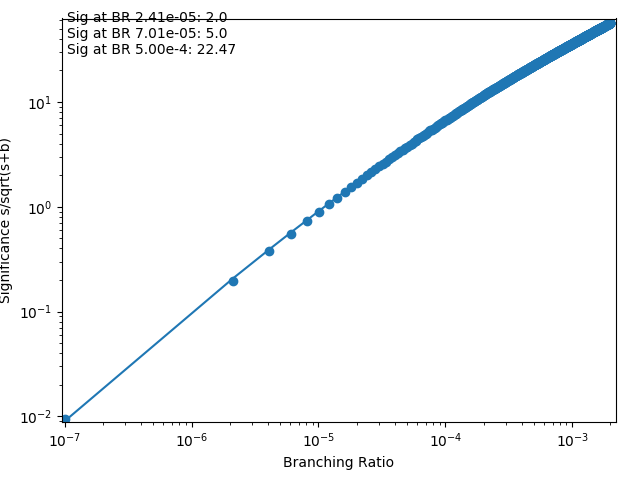
\includegraphics[width=0.85\textwidth]{Images/ejetsOuts/SigVsBR.png} 
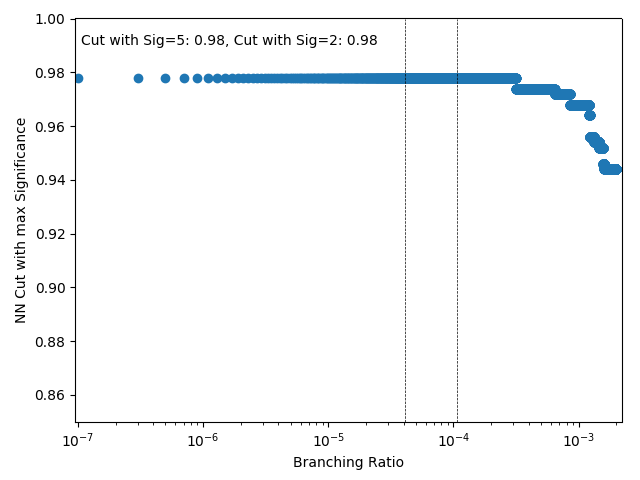
\includegraphics[width=0.85\textwidth]{Images/ejetsOuts/CutVsBR.png} 
\end{column}
\end{columns}
}

\frame{\frametitle{Significance Plots, Muon Channel}
\begin{columns}
\begin{column}{0.48\textwidth}
\centering
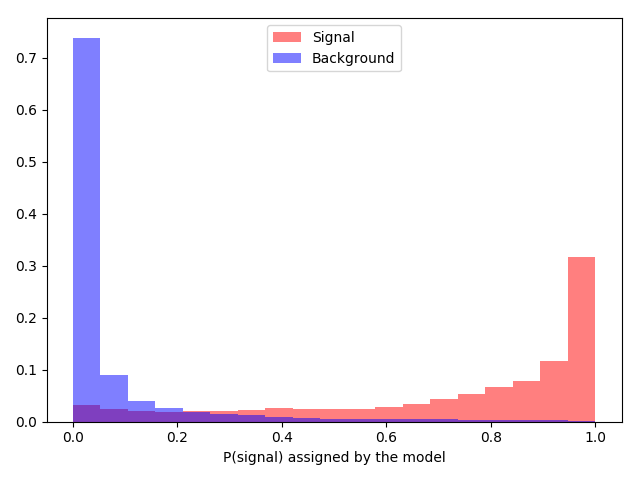
\includegraphics[width=0.85\textwidth]{Images/mujetsOuts/sigbkg.png} 
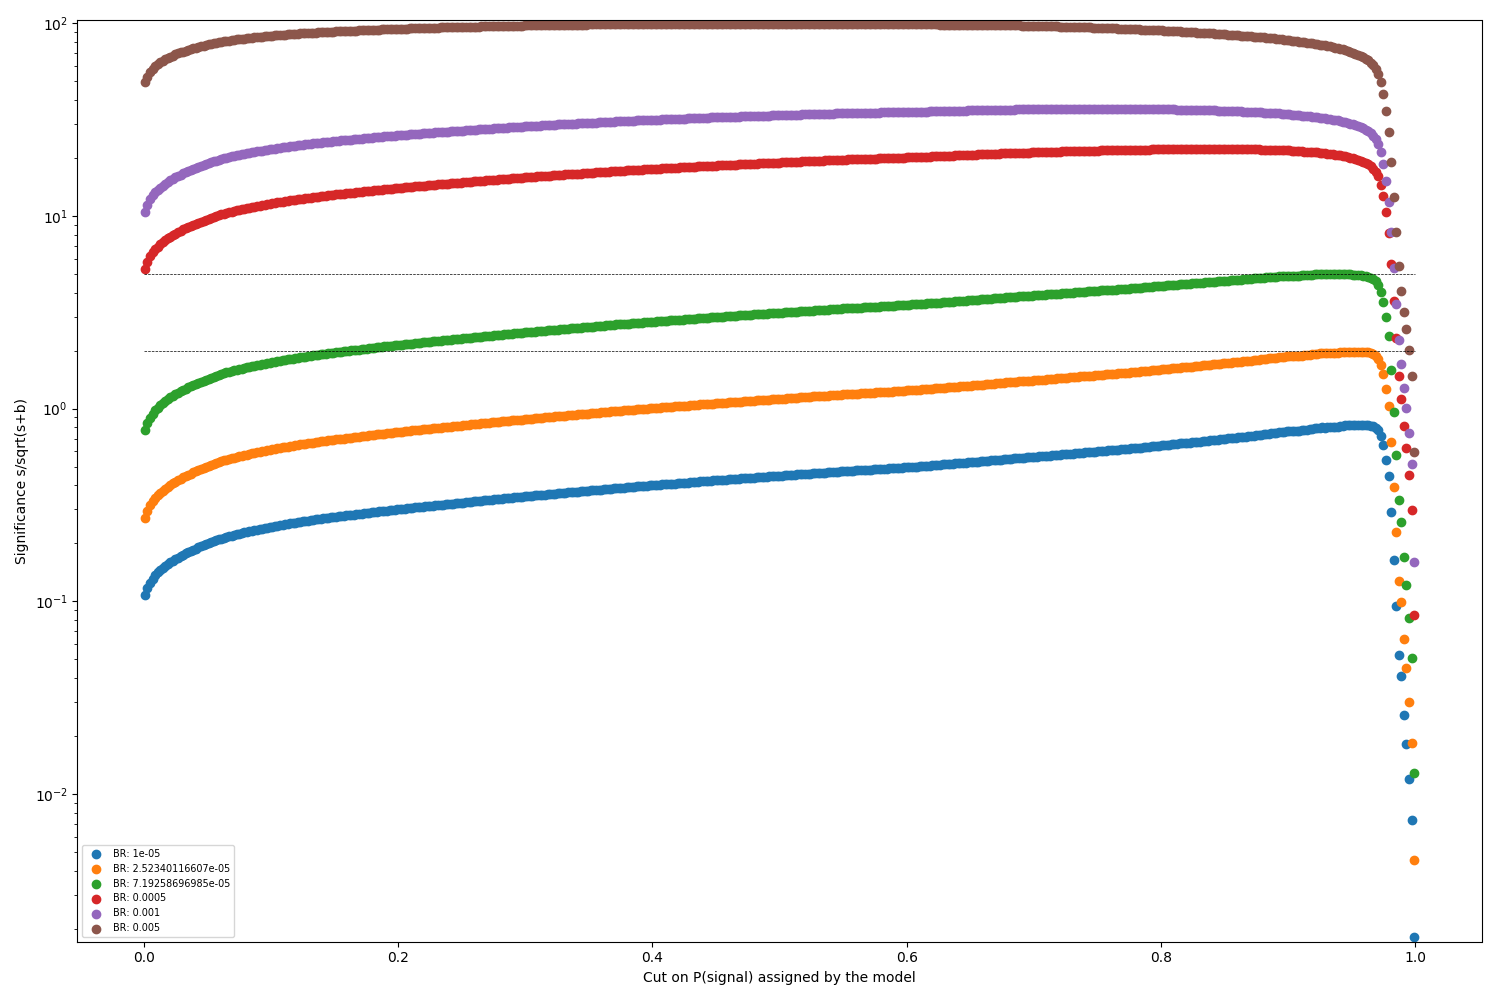
\includegraphics[width=0.85\textwidth]{Images/mujetsOuts/significance2.png} 
\end{column}
\begin{column}{0.48\textwidth}
\centering
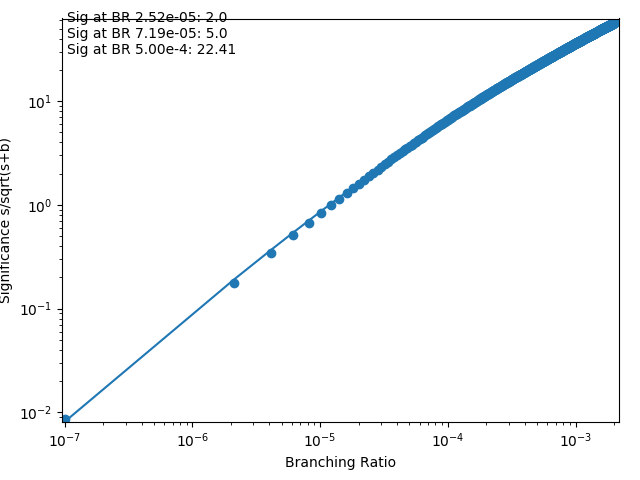
\includegraphics[width=0.85\textwidth]{Images/mujetsOuts/SigVsBR.png} 
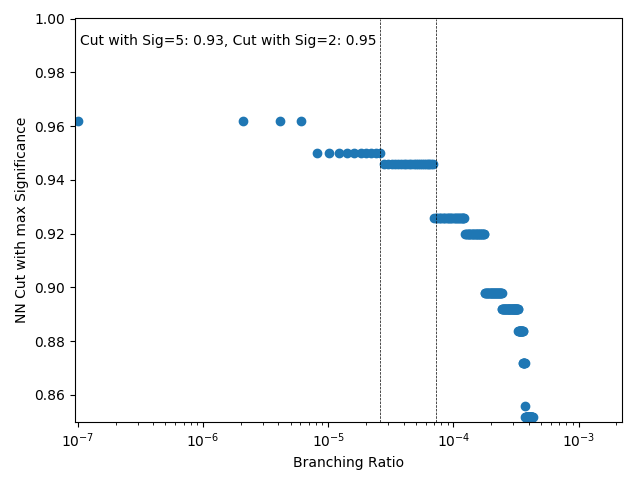
\includegraphics[width=0.85\textwidth]{Images/mujetsOuts/CutVsBR.png} 
\end{column}
\end{columns}
}


%%%%%%%%%%%%%%%%%%%%%%%%%%%%%%%%%%%%%%%%%%%%%

\section{Continuing Analysis}
\subsection{Region Creation}
\frame{\frametitle{Control and Validation Regions}
\begin{itemize}
\item Validation and Control Regions are created orthogonal to Signal Region for large backgrounds
\item VR for ($t\bar{t}+\gamma$), ($W+\gamma$)
\item CRs for regions without real photons
\begin{itemize}
\item These regions include $t\bar{t}$ and $W$ rich samples with 0 good photons, so many events new regions should probably be created
\end{itemize}
\item Previous cuts to make these regions make less sense to do now with NN Cuts
\end{itemize}
}

\subsection{New Ntuple Production}
\frame{\frametitle{New Ntuple Production}
\begin{itemize}
\item New tools have been recently developed in the Top Group (VGammaORTool, Duplicate Event Removal)
\item Replacing Custom Event Saver with that of tt+gamma group, more support and faster integration of new tools
\item Custom post-grid local processing code developing
\item Will transition with the currently running ntuples to local mini-ntuple creation
\item Beginning to work with TRExFitter to push toward the statistical part of the analysis
\end{itemize}
}
%%%%%%%%%%%%%%%%%%%%%%%%%%%%%%%%%%%%%%%%%%%%%%%%%%%%%%%%%%%%%%%%%%
\section{Outlook and Conclusions}

\frame{\frametitle{Outlook}
\begin{itemize}
\item Still lots to be done
\item Fake Rates $e\rightarrow\gamma$ and $j\rightarrow\gamma$ to be investigated
\item Using full MC16a/Data15,16 for quick iterations, have access to full MC/Data sets 
\item Happy with the state of the neural network studies, any further reduction would require significant time for insignificant gain \\
\item Questions?
\end{itemize}
}



%%%%%%%%%%%%%%%%%%%%%%%%%%%%%%%%%%%%%%%%%%%%%%%%%%%%%%%%%%%%%%%%

\appendix
\section{Backup}
\frame{\frametitle{Backup}
}
\frame{\frametitle{FCNC Diagrams}
\centering
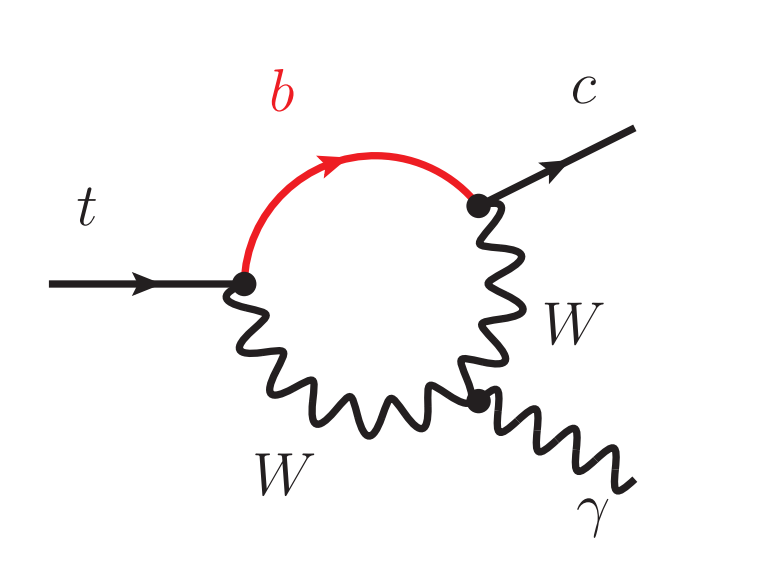
\includegraphics[width=.4\textwidth]{../../Thesis/ThesisImages/FCNCLoop.png}
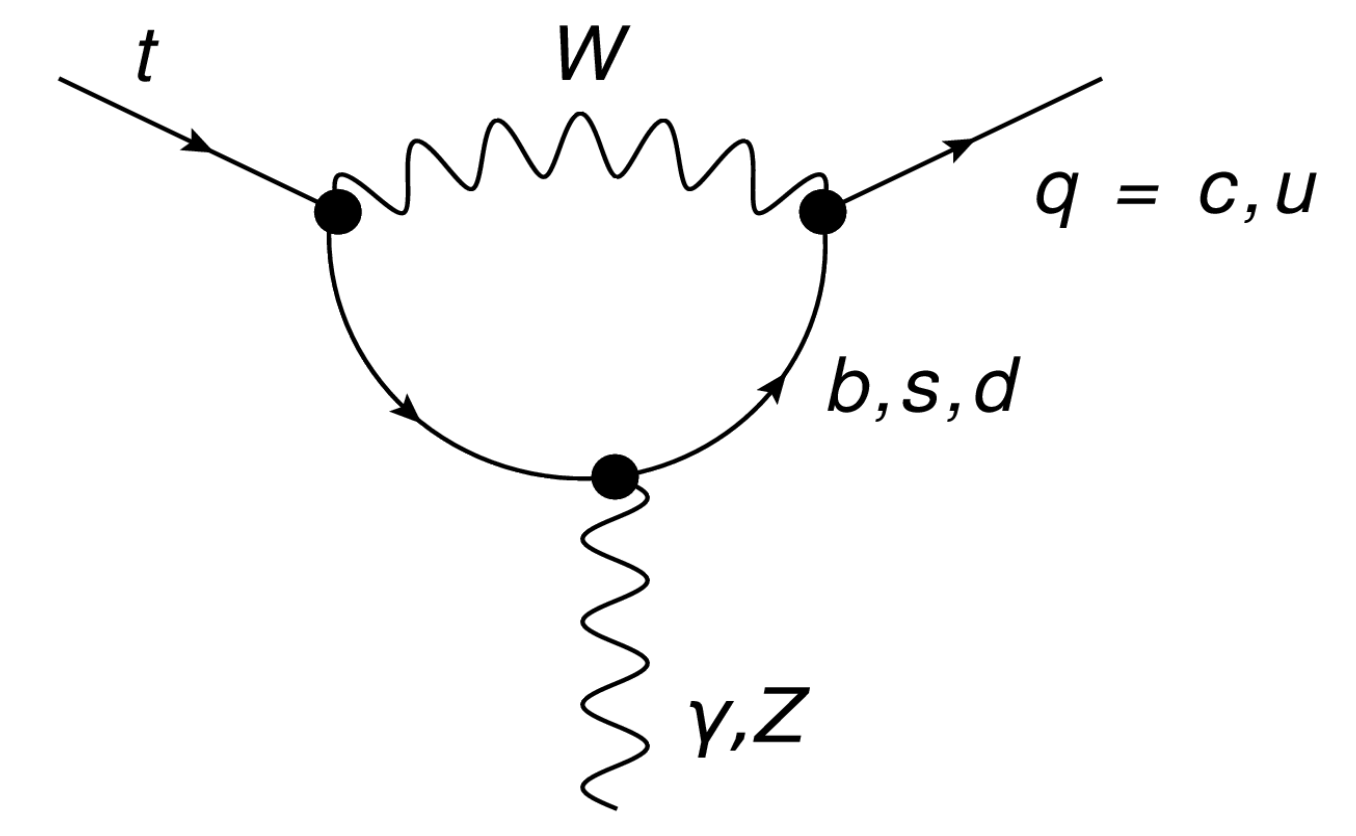
\includegraphics[width=.4\textwidth]{../../Thesis/ThesisImages/penguinFCNC.png}
}

\frame{\frametitle{NN Input Variable Correlations}
\centering
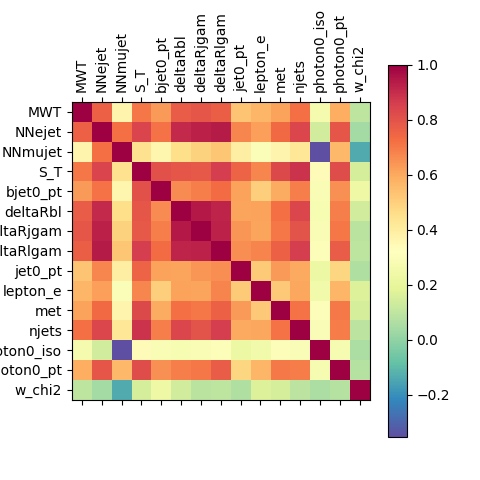
\includegraphics[height=.8\textheight]{Images/correlations.png}
}

\frame{\frametitle{Neural Network Model Inputs}
\centering
\scalebox{0.8}{ $\text{Separation} = \sum_{i}^{bins} \frac {n_{s i}-n_{b i}}{n_{s i}+n_{b i}}$}
\begin{columns}
\begin{column}{0.48\textwidth}
\centering
mu+jets channel\\
\scalebox{0.6}{\begin{tabular}{cc}
Variable & Separation \\
\hline
photon0iso & 41.18 \\
mqgam & 28.27 \\
photon0pt & 24.07 \\
mtSM & 11.60 \\
mlgam & 7.56 \\
deltaRjgam & 5.64 \\
deltaRbl & 4.42 \\
MWT & 3.34 \\
ST & 3.30 \\
nuchi2 & 3.12 \\
jet0pt & 2.81 \\
njets & 2.07 \\
smchi2 & 1.89 \\
wchi2 & 1.87 \\
jet0e & 1.52 \\
deltaRlgam & 1.17 \\
leptone & 0.87 \\
deltaRjb & 0.86 \\
met & 0.68 \\
bjet0pt & 0.52 \\
leptoniso & 0.27 \\
\end{tabular}
}
\end{column}
\begin{column}{0.48\textwidth}
\centering
e+jets channel \\
\scalebox{0.6}{\begin{tabular}{c c}
Variable & Separation\\
\hline
photon0pt & 23.14 \\
mqgam & 22.73 \\
photon0iso & 18.70 \\
mtSM & 11.02 \\
mlgam & 9.53 \\
deltaRbl & 5.00 \\
deltaRjgam & 4.60 \\
ST & 3.83 \\
MWT & 3.16 \\
jet0pt & 2.47 \\
njets & 1.70 \\
nuchi2 & 1.59 \\
deltaRlgam & 1.40 \\
wchi2 & 1.33 \\
smchi2 & 1.09 \\
deltaRjb & 0.88 \\
leptone & 0.85 \\
leptoniso & 0.56 \\
bjet0pt & 0.50 \\
met & 0.47 \\
\end{tabular}
}
\end{column}
\end{columns}
}

\frame{\frametitle{Input Variables}
['photon0iso','photon0pt','mqgam','mlgam','mtSM','deltaRjgam','deltaRbl',\\
'MWT','ST','njets','wchi2','jet0pt','deltaRlgam','leptone','met','bjet0pt']


}

\frame{\frametitle{Integrated Luminosity}
\centering
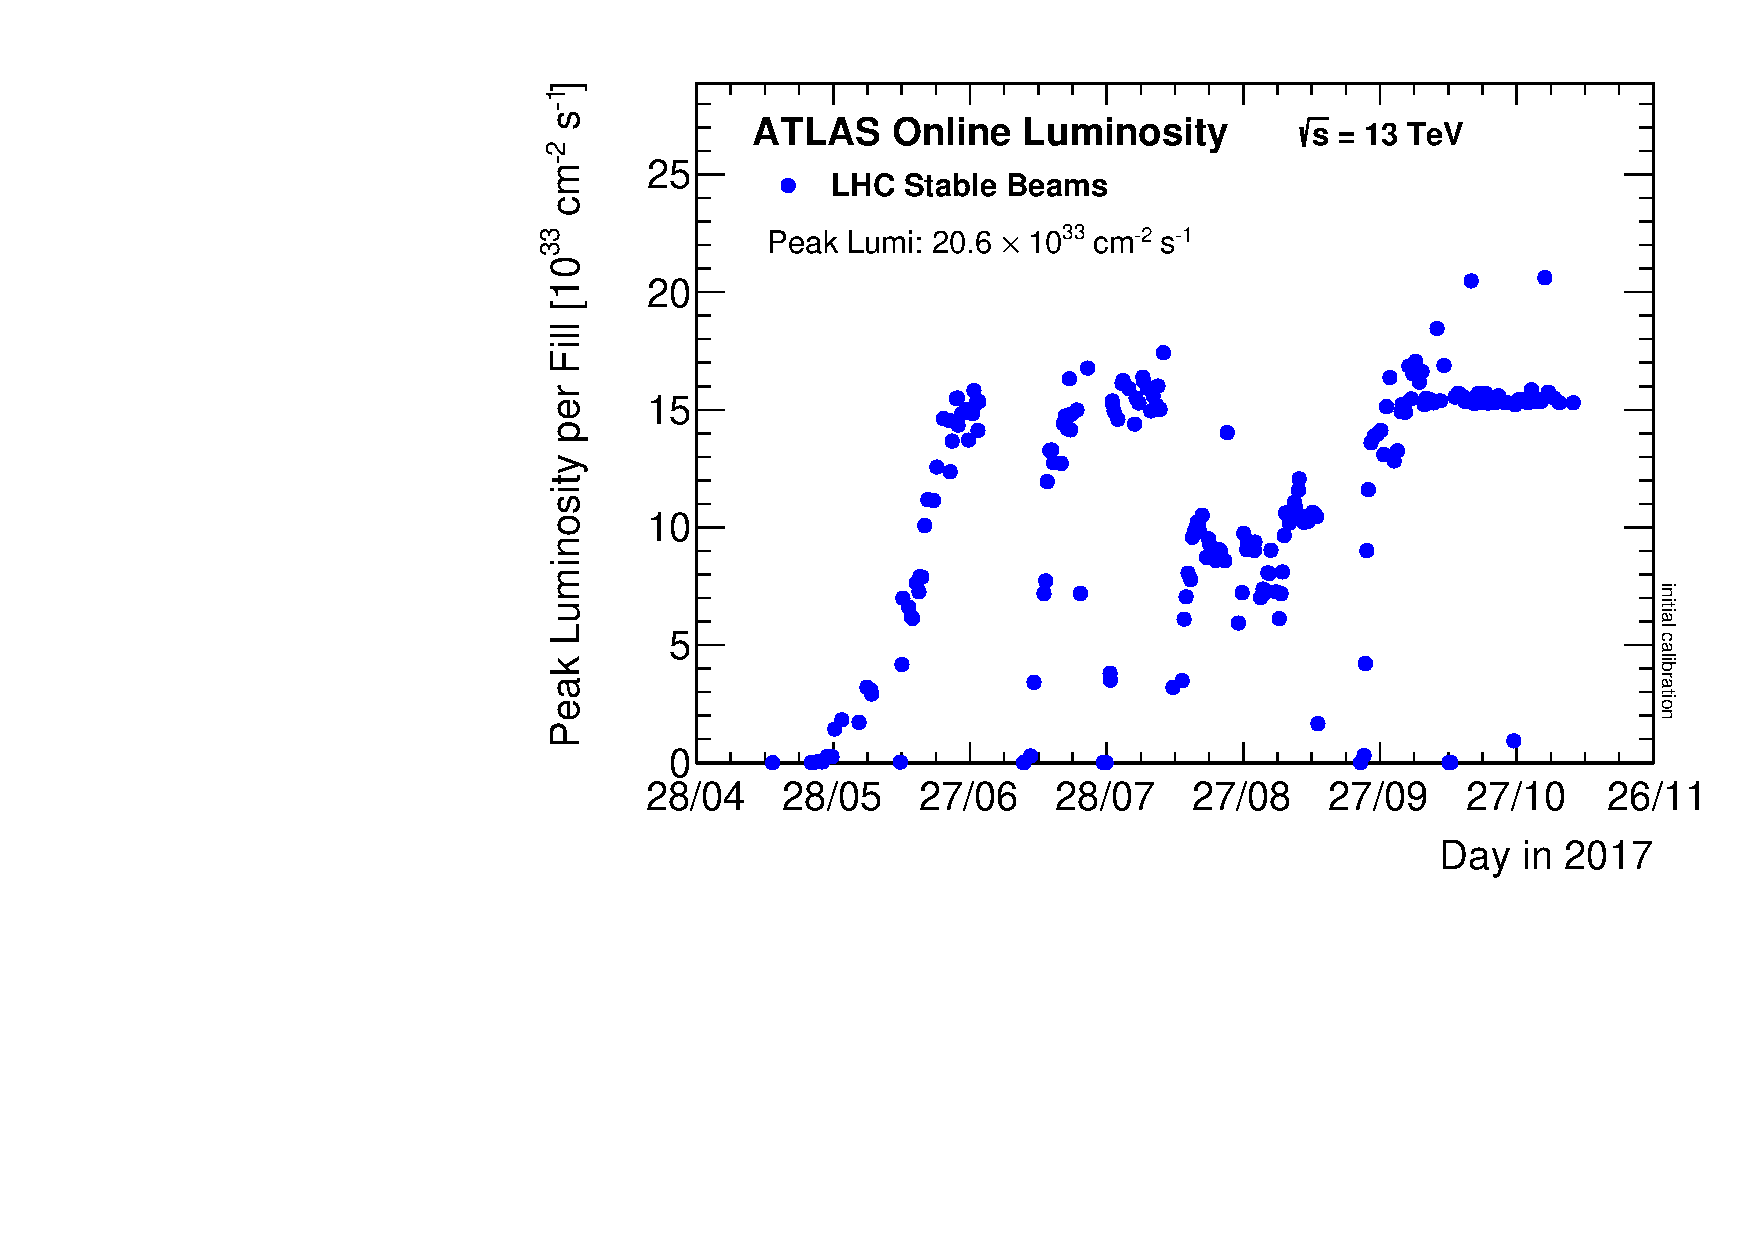
\includegraphics[width=1.\textwidth]{../../Thesis/ThesisImages/2017PeakLumiByFill.pdf}
}
\frame{\frametitle{A Couple BSM Diagrams}
\centering
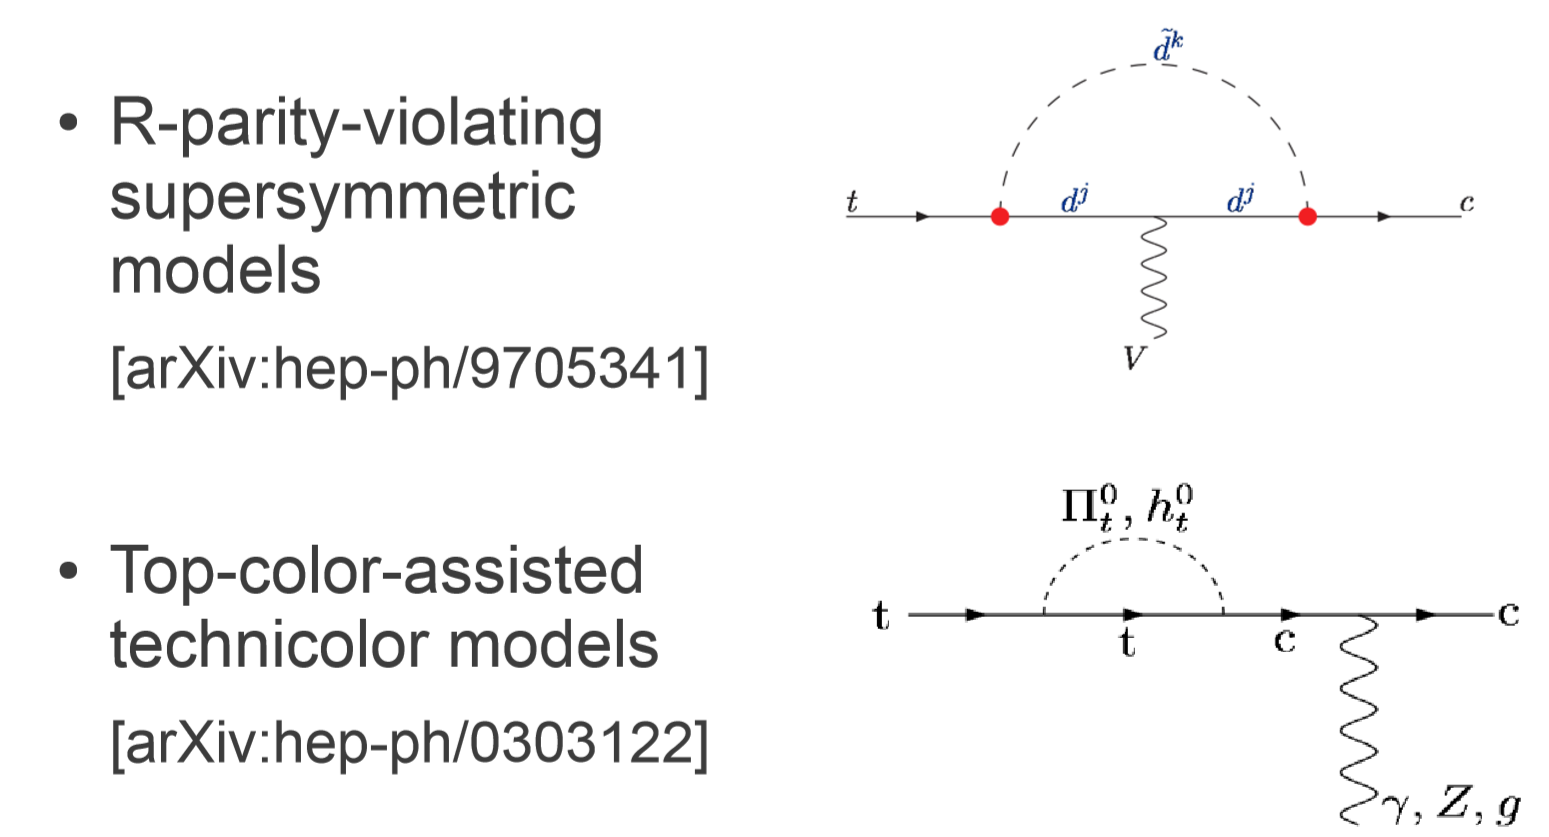
\includegraphics[width=1.\textwidth]{../../Thesis/ThesisImages/BSMDiagrams.png}
}

\frame{\frametitle{Jets/AntiKT}

\[ d_{ij} = min(\frac{1}{p_{ti}^2},\frac{1}{p_{tj}^2}) \frac{\Delta_{ij}^2}{R^2}
\]
\[ d_{iB} = \frac{1}{p_{ti}^2}
\]
\[ \Delta_{ij}^2 = (\eta_i -\eta_j )^2 + (\phi_i - \phi_j )^2
\]
\begin{itemize}
\item Find minimum of entire set of $\{ d_{ij},d_{iB} \}$
\item If $d_{ij}$ is the minimum particles i,j are combined into one particle and removed from the list of particles
\item If $d_{iB}$ is the minimum i is labelled as a final jet and removed from the list of particles
\item Repeat until all particles are part of a jet with distance between jet axes $\Delta_{ij}$ is greater than R
\end{itemize}
}

\frame{\frametitle{B-tagging}
\centering
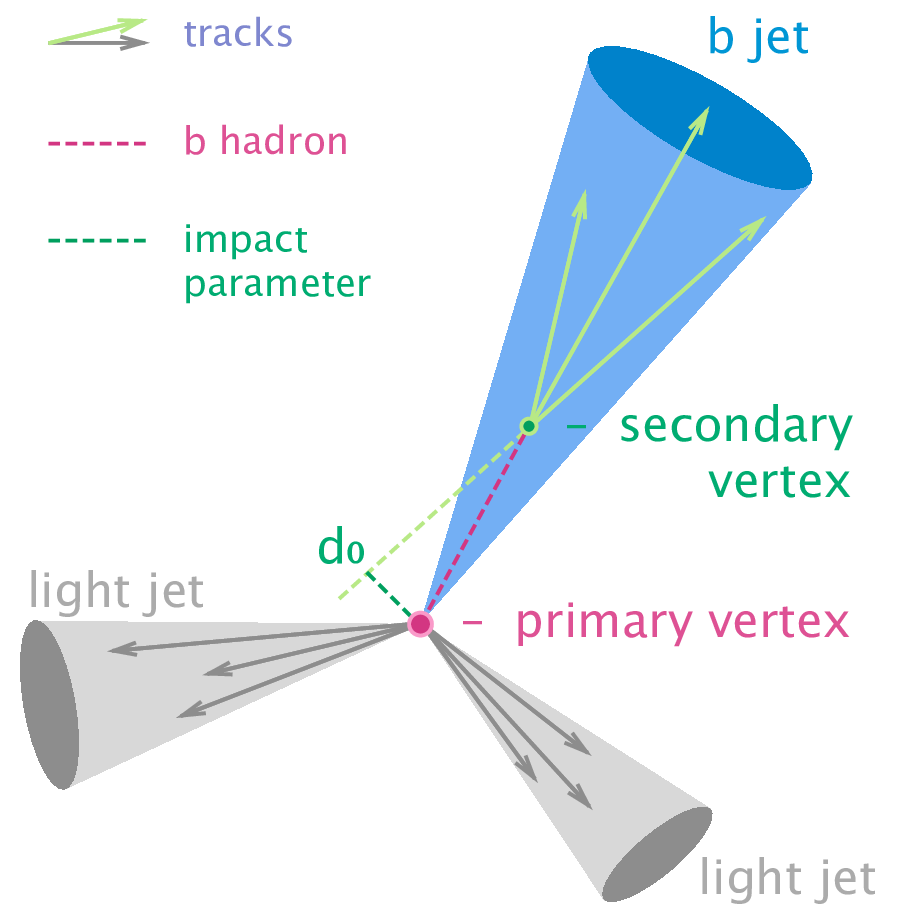
\includegraphics[height=.8\textheight]{../../Thesis/ThesisImages/B-tagging_diagram.png}
}

\frame{\frametitle{}
\[ \mathcal{L}^{eff}_{tq\gamma} = - e \bar{c} \frac{i \sigma^{\mu\nu}q_{\nu}}{m_t}(\lambda^{L}_{ct}P_L + \lambda^{R}_{ct}P_{R}) t A_{\mu} +H.c.
\]
}

\end{document}

%36.070


%%% Neural Net Ref: http://cs231n.github.io/neural-networks-1/

% npart0=['photon0_iso','photon0_pt','m_qgam','m_lgam','m_tSM','deltaRjgam','deltaRbl','MWT','S_T','nbjets','njets','w_chi2','jet0_pt','nu_chi2','sm_chi2','deltaRlgam','lepton_e','met','lepton_iso','bjet0_pt']
%all vars

%npart = ['photon0_iso','photon0_pt','m_qgam','m_lgam','m_tSM','deltaRjgam','deltaRbl','MWT','S_T','njets','nbjets','w_chi2','jet0_pt','deltaRlgam','lepton_e','met','bjet0_pt']
%usual npart1

%npart1=['photon0_iso','photon0_pt','deltaRjgam','deltaRbl','MWT','S_T','njets','w_chi2','jet0_pt','deltaRlgam','lepton_e','met','bjet0_pt']
%minimal